% Created November 2014 by Carl D. Sorensen
% Modified October 2019 by Brian D. Jensen

\documentclass[letterpaper, 11pt, twoside, article]{memoir}


%%% REVISION INFORMATION
%%% Set the date and revision number below to the correct values
\newcommand{\revdate}{18 Nov. 2019}
\newcommand{\revnum}{1.0}

%%% The material below should only be modified if you know what you're doing with it!
\setstocksize{11in}{8.5in}
\setlrmarginsandblock{1.5in}{1in}{*}

\setulmarginsandblock{1in}{1in}{*}

\checkandfixthelayout[classic]

\usepackage[T1]{fontenc}

%\usepackage{fontspec}
\usepackage{graphicx}
\usepackage{booktabs}
\usepackage{enumitem}
\usepackage{xcolor, colortbl}
\usepackage{array}
\usepackage{calc}
\usepackage[font=small,singlelinecheck=false]{caption}
\usepackage{pdfpages}
\usepackage{mathptmx}
\usepackage[hidelinks]{hyperref}

% Degree symbol
\usepackage{gensymb}
\usepackage{float}

% Add new lists -- Primary Artifacts and Supporting Artifacts
%
%% Primary Artifacts
\newcommand{\primaryartifactname}{Primary Artifacts}
\newlistof{listofprimaryartifacts}{pa}{\primaryartifactname}
\newcounter{primaryartifact}[chapter]
\newlistentry{primaryartifact}{pa}{0}
\renewcommand{\theprimaryartifact}{\arabic{primaryartifact}}
\newcommand{\primaryartifact}[1] {
  \refstepcounter{primaryartifact}
  \addcontentsline{toc}{primaryartifact}{\hspace{1.5em}#1}
  \addcontentsline{pa}{primaryartifact}{\hspace{1.5em}#1}
  }
\cftpagenumbersoff{primaryartifact}  

%% Supporting Artifacts
\newcommand{\supportingartifactname}{Supporting Artifacts}
\newlistof{listofsupportingartifacts}{sa}{\supportingartifactname}
\newcounter{supportingartifact}[chapter]
\newlistentry{supportingartifact}{sa}{0}
\renewcommand{\thesupportingartifact}{\arabic{supportingartifact}}
\newcommand{\supportingartifact}[1] {
  \refstepcounter{supportingartifact}
   \addcontentsline{toc}{supportingartifact}{\hspace{1.5em}#1}
   \addcontentsline{sa}{supportingartifact}{\hspace{1.5em}#1}
  }
\cftpagenumbersoff{supportingartifact}  


% Trick for fixed-width table columns
\newcolumntype{L}[1]{>{\raggedright\let\newline\\\arraybackslash\hspace{0pt}}p{#1}}
\newcolumntype{C}[1]{>{\centering\let\newline\\\arraybackslash\hspace{0pt}}p{#1}}
\newcolumntype{R}[1]{>{\raggedleft\let\newline\\\arraybackslash\hspace{0pt}}p{#1}}

% Fractional Width columns
\newcolumntype{z}[1]{>{\hsize=#1\hsize\raggedright\arraybackslash}X}
\newcolumntype{a}[1]{>{\hsize=#1\hsize\raggedleft\arraybackslash}X}
\newcolumntype{q}[1]{>{\hsize=#1\hsize\centering\arraybackslash}X}

%%% This ends the material you should only modify if you know what you're doing.


%%%%% adjust spacing -- Choose one line to uncomment

%\abnormalparskip{0.5\baselineskip}  %adjusts spacing between paragraphs under user control
%\nonzeroparskip  % Default value for non-zero spacing between paragraphs
\traditionalparskip  % No extra spacing between paragraphs -- recommended by Wilson, the author of the memoir class



\begin{document}

\raggedright

\frontmatter

%You should comment out or erase the page below to make your package.


% This document provides help on creating your Concept Design Report. It includes a sample title page and representative headings for the Design Summary, which can also be inserted as a pdf file. We are providing this template as a suggestion to help your team create a high quality Concept Design Report. The template includes suggestions for layout and formatting so that you don't have to worry about figuring these details out. You can and should adapt the contents of the report \emph{as appropriate for your project.}

% You do not need to include all of the representative sections. You may include additional sections. Your decisions about what to include should be guided by the desire to communicate clearly and concisely.

% The artifacts listed in the Primary Artifacts and Secondary Artifacts sections are typical, but your project may require different
% artifacts.  Use appropriate artifacts for your project.

% Please refer to the Evaluation rubric for the Concept Development Stage Approval Package (see Stage Approval: Concept Development in the Capstone Reference) for information about how the report will be evaluated. Hopefully, these guidelines will help you better understand the rubric. If you have questions, please ask.

% The formatting of your report is largely up to your team. You must allow a 1 inch margin on all unbound edges, and a 1.5 inch margin on the bound edge. You may use either single- or double-sided printing. If you have no preference, we suggest you print double-sided.  Please refer to Stage Approval: Concept Development in the Capstone Reference for detailed formatting requirements.

% We recommend that your document be largely in black and white.  Color will cost more to print and the color printers have lower capacity (in terms of pages per minute) than the black and white printers; this will affect you at the end of the semester when everyone is trying to print at the same time.

% NOTE: THIS TITLE PAGE SHOULD NOT BE PART OF YOUR STAGE APPROVAL PACKAGE.  THE TEMPLATE BEGINS ON THE NEXT PAGE.


\cleardoublepage
%This is the end of the material to erase.

\begin{centering}
\thispagestyle{empty}

{\Huge Concept Design Report}

\Large
\vspace{0.5in}
\revdate\\
Revision \revnum
\vspace{0.5in}

% Replace the line below with your project title
Tracker for In-Flight Air Vehicle\\
\vspace{0.5in}

Project Sponsor: \\
 IMSAR

\vspace{0.5in}

% logo

\includegraphics[width=.2\textwidth]{Not_Artifacts/Logo_Image/logo_navy.png}

\vspace{0.4 in}

Capstone Team 15: RPS


\normalsize

\vspace{1.6 in}

%\begin{centering}

\Large

Ira A. Fulton College of Engineering \\
Brigham Young University

\end{centering}


\clearpage

\chapter*{Revision History}

\begin{tabularx}{\textwidth}{|q{.3}|q{.5}|z{2.2}|}
\hline
Revision & Date & Description  \\
\hline
1.0 & 11 Nov.\ 2019 & Initial draft, based on previous year's template \\
\hline
\end{tabularx}

\cleardoublepage

\begin {centering}
{\LARGE Approval Signatures}

\vspace{.5in}

The undersigned certify that they have read the Concept Design Report and that it is a true and accurate representation of the project.

\end{centering}
\vspace{.5 in}			
\begin{tabularx}{\textwidth}{C{.25 in} L{2.5 in} C{.5 in} R{1.5 in}}
\cline{2-2} \cline {4-4}

& Autumn Twitchell & & Date \vspace{.25 in}\\
\cline{2-2} \cline {4-4}
& Daniel Sharp & & Date \vspace {.25 in}\\
\cline{2-2} \cline {4-4}
& Garret Gang & & Date \vspace{.25 in}\\
\cline{2-2} \cline {4-4}
& Jesse Krage & & Date \vspace{.25 in}\\
\cline{2-2} \cline {4-4}
& Joe Hansen & & Date \vspace{.25 in}\\
\cline{2-2} \cline {4-4}
& Nicholas Merriman & & Date \vspace{.25 in}\\
\cline{2-2} \cline {4-4}
&  Larkin Hastriter - Team Coach & & Date \vspace{.25 in}\\
\cline{2-2} \cline {4-4}
& Mark Catanzaro - IMSAR & & Date \vspace{.25 in}\\
\cline{2-2} \cline {4-4}
& Brian Jensen - Project Instructor & & Date \vspace{0 in}\\

\end{tabularx}

\vspace{1 in}

\cleardoublepage

\tableofcontents*


\mainmatter

%% If you want to insert the Design Summary as a pdf file, uncomment the lines below, and delete or comment out all of the Design Summary text.
%\addcontentsline{toc}{chapter}{Design Summary}
%\includepdf[pages=-]{DESIGN_SUMMARY_NAME.pdf}

\addcontentsline{toc}{part}{Design Summary}

The first 2--4 pages of the Concept Design Report contain the Design Summary, whose main elements are described here.  The Design Summary should not be more than 4 pages; you will have to work hard to get an excellent Design Summary, because there's not much space!


\chapter{Introduction}

IMSAR is a local company that specializes in making compact radar systems more affordable and accessible for use in small air vehicles. One of the stationary ground systems currently produced and sold by IMSAR is a computer-controlled tilt and pan positioner that maintains a communication link with radar units installed on air vehicles. The operational situation for these units is to be in a stationary position 2 to 20 miles away from the target in-flight vehicle. The current design employs a tilt and pan positioner that has become obsolete. Our team has been tasked with replacing the tilt and pan positioner, installing an onboard computer, and creating control software necessary to maintain a communication link.  

~\\

Our team’s objective is to design, prototype, and test a Radar Positioning System (RPS) that can track in-flight vehicles while maintaining visual contact by March 30, 2020 for under \$1,500 and 1,500 man-hours. The overall performance of the system will be evaluated based on the following key success measures: time to train the user, percent increase in target acquisition time from minimum acquisition time, and the initial setup time. Ultimately the amount of time that the aircraft is within the field of view (i.e. the percent of time that a communication link is maintained) is the most important criteria. IMSAR’s current system maintains a communication link 100\% of the time under normal use conditions. Thus, we have determined that it is necessary for our end product to also maintain a communication link 100\% of the time. Because this is a binary success or failure, it is not included in the key success measures, however, it is the most important criteria for the system. Full system requirements can be found in the requirements matrix (RM-001) attached to this document. 

 ~\\

During the concept development stage three primary subsystems were defined i.e. the user interface, the system architecture, and the tracking method. Concepts for each of these subsystems were developed, and decisions on which concepts to pursue were made.

%The introduction is a place to present the problem to be solved in broad terms.
%It may be helpful to briefly discuss the project sponsor and how solving the problem will advance the goals of the sponsor.
%You may wish to include your Project Objective Statement here.
%The introduction should summarize the most important market requirements, performance measures, ideal values, and target values, including the key success measures. You will likely wish to refer to the project contract and the system requirements matrix artifacts.
%After reading this section, the reader should clearly understand the most important performance goals for your product.
%Tables will likely help to clearly and succinctly communicate your requirements. 


\chapter{Selected Concepts and their Justification}

\textbf{User Interface Selected Concept} 

~\\
We have decided to develop a web-based user interface to setup the communication link. The user interface will allow the operator to input initialization parameters including the LLA and heading bias of the communication link, and the LLA of the aircraft or the relative position of the aircraft depending on which is known. The goal of the user interface is to be as intuitive as possible and require minimal training while still offering full functionality. See artifact XXXXX for user interface details. 

~\\

\textbf{Justification for User Interface Concept} 

 ~\\
Having a web-based user interface will allow the user to use their own device to setup the communication link. This will make the system easier to use and lead to a more desirable product. An initial layout was made using PowerPoint, then taken to the user experience club at BYU for feedback. Updates to the layout were made based on the feedback received. After several iterations the layout was shown to Mark Catanzaro and Daniel Gunyan of IMSAR for more feedback. After meeting with them we were able to identify the critical features and make further updates. Based on their feedback we are confident that the user interface will be capable of meeting the requirements.

~\\
\textbf{Tracking Method Selected Concept} 

 ~\\
The team has decided to use a reactionary method to track the aircraft. The aircraft will broadcast a health message including its location at a rate of about 2 Hz. When the communication link receives the LLA coordinate of the drone, the dish will move to point at that location.  

~\\
\textbf{Justification for Tracking Method} 

 ~\\
To justify using a reactionary method as opposed to a predictive method we wrote a Python script that simulates a vehicle in flight. For the simulation we had the drone flying a half mile away from the positioner at a speed of 60 mph. Note that this distance is closer than the nearest distance that will be used in real life. For the simulation we had the drone constantly moving with a box representing an 8\degree field of view updating its location at a rate of 2 Hz. This allowed us to visualize how quickly the aircraft would leave the field of view and if an update rate of 2 Hz could feasibly track it. In our testing the drone was easily maintained within the field of view. For more details on the testing see artifact XXXX.  

 ~\\
It should also be noted that the current system produced and used by IMSAR also uses a reactionary control method. They are able to maintain a communication link using this method. Because this method has been shown to work and our own simulation supports this, we are confident that this approach will lead to a functioning and desirable end product.  

~\\
\textbf{System Architecture Selected Concept} 

 ~\\
We have decided to use a Raspberry Pi 3 to host a web server and run the necessary software to drive the positioner. This approach will allow the user to access the GUI from their own machine so long as they are on the same network as the Pi. Communication between the server and control software will be accomplished with a “single producer single consumer” queue. This will allow the server to write to this queue and the controller to read to the queue. This will maximize the rate of information throughput while still ensuring that the setup is thread safe. That is, the communication between the server and controller will not have any unintended interactions.   

 ~\\
The latency for this communication setup is consistently less than 3ms, which is well under the necessary time threshold.   

~\\
\textbf{Justification for System Architecture} 

 ~\\
In our early meetings with IMSAR, we discussed the possibility of hosting a browser-based GUI on a Raspberry Pi. They were thrilled with this possibility. They liked the convenience of having an easily accessible GUI and the flexibility of the Raspberry Pi. Our testing showed that this design is not only plausible for accomplishing the design requirement, but exceptional. We developed a working version of the system in action to validate its credibility.   

%This section of the Design Summary gives a summary description of the product as currently defined. It provides a summary of the answer to stage approval question 1  ``What is the selected concept?''. It is not expected to provide the complete answer to the question, which would be answered by the design package artifacts.
%Generally, photographs, renderings, sketches, block diagrams, and similar kinds of images will be helpful in conveying the product description.
%If you choose to use photographs, do your best to make them high-quality photographs. It is generally better to include people in the photographs. You should always be aware of the background. Eliminating clutter in the background (or foreground) of your photographs will help them communicate better.

%This section of the Design Summary provides a summary of the answer to stage approval question 2, ``How have your proven that your concept is best and meets the key success measures and other requirements?'' 
%It summarizes methods you have used that demonstrate your chosen concept is judged to be the best among a relatively large number of concepts. You should refer to one or more concept selection artifacts for more details.
%It also summarizes how well the system has been demonstrated to perform through tests applied to prototypes and models. You should refer to artifacts that define the prototypes and models, the test procedures, and the results.
%Tables can be effective methods for communicating the performance testing results, particularly for tests related to the key success measures.

   
\addtocontents{toc} {
\cftpagenumbersoff{chapter}  % turn off page numbers in TOC
\cftpagenumbersoff{section}
}

\cleardoublepage
\pagestyle{empty}


\listofprimaryartifacts
\thispagestyle{empty}
\clearpage

% \cleardoublepage  %%% Used if including pdf artifacts directly
\primaryartifact{CD-001 Concept Definition}  
%% To include a pdf file of the artifact, uncomment the line below, and put the name of the pdf in the correct spot.
%   \includepdf[pages=-]{NAME-OF-PDF}  % Includes all pages of a pdf file

% \cleardoublepage  %%% Used if including pdf artifacts directly
\primaryartifact{CS-001 Concept Selection Report}  
%% To include a pdf file of the artifact, uncomment the line below, and put the name of the pdf in the correct spot.
%   \includepdf[pages=-]{NAME-OF-PDF}  % Includes all pages of a pdf file

% \cleardoublepage  %%% Used if including pdf artifacts directly
\primaryartifact{RM-001 Requirements Matrix}  
%% To include a pdf file of the artifact, uncomment the line below, and put the name of the pdf in the correct spot.
%   \includepdf[pages=-]{NAME-OF-PDF}  % Includes all pages of a pdf file

% \cleardoublepage  %%% Used if including pdf artifacts directly
\primaryartifact{CT-001 Concept Testing Report}  
%% To include a pdf file of the artifact, uncomment the line below, and put the name of the pdf in the correct spot.
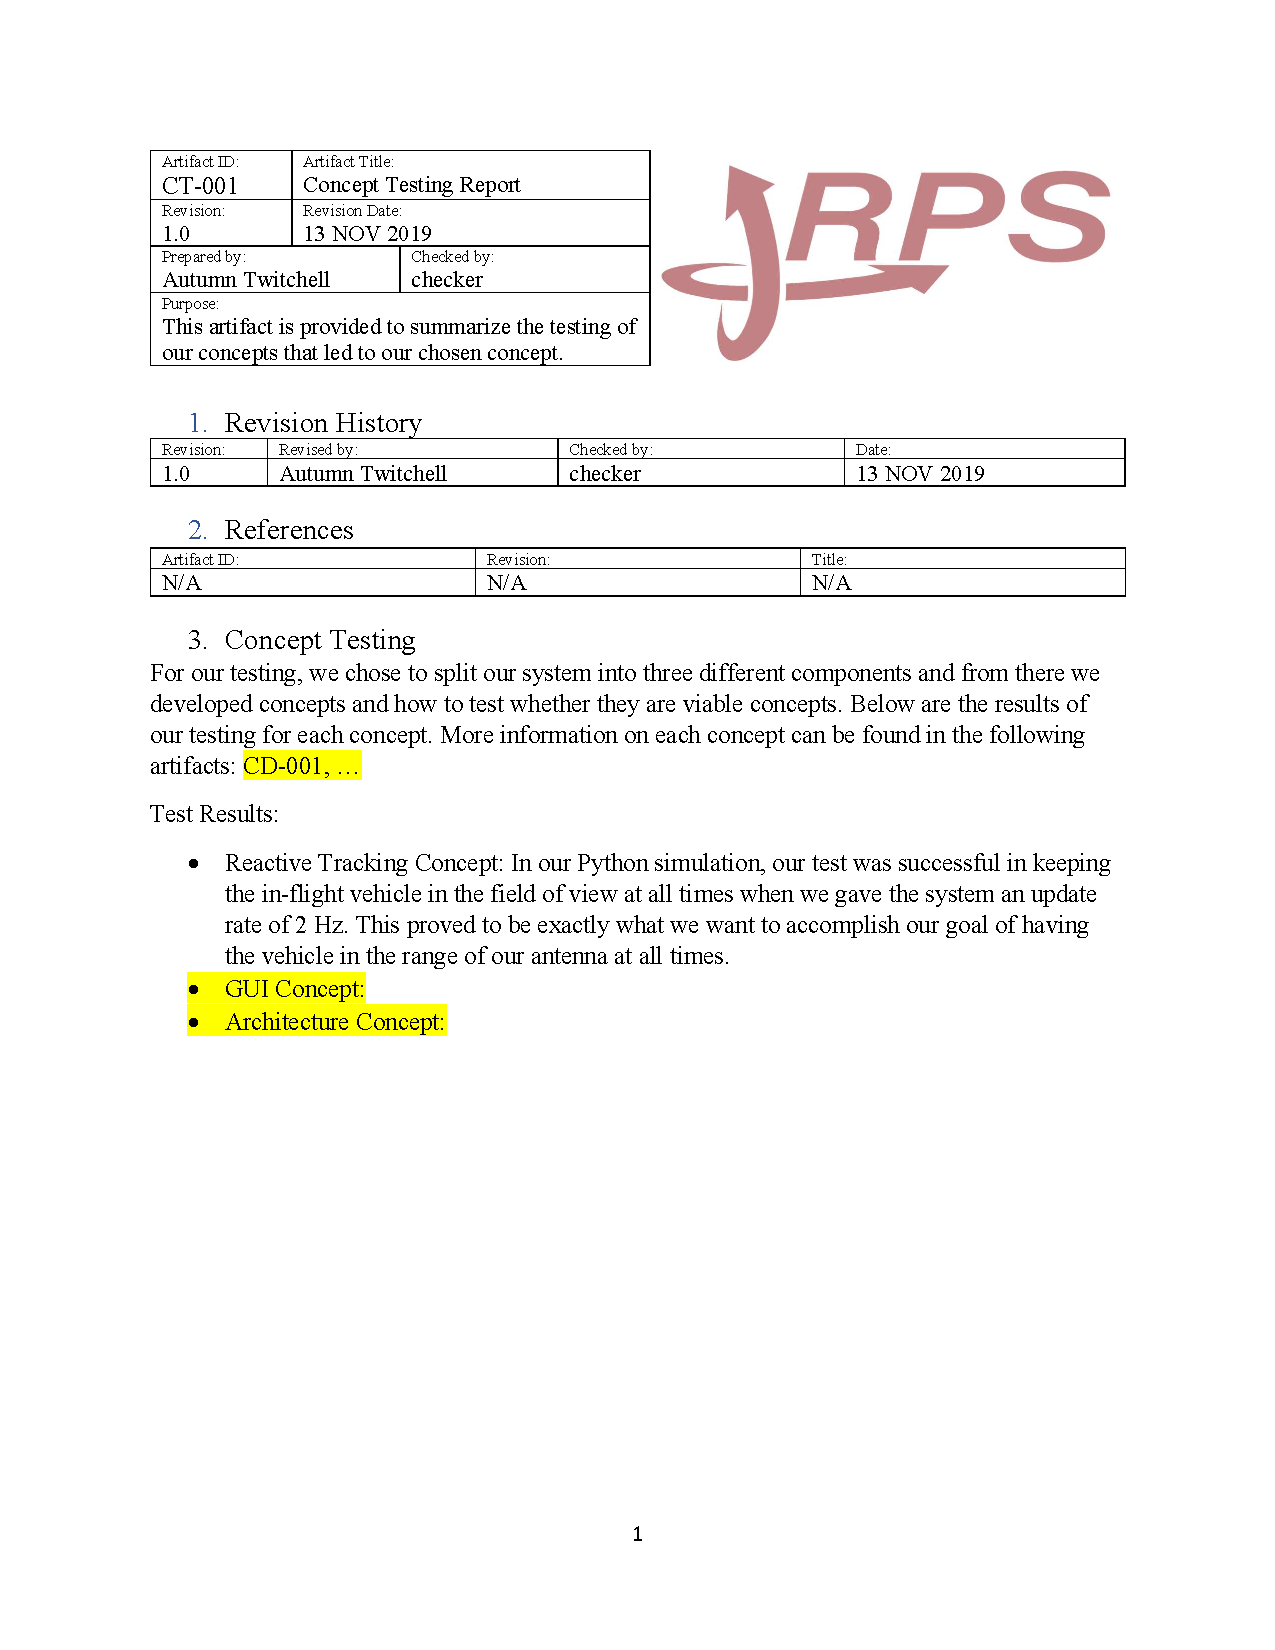
\includepdf[pages=-]{Artifacts/CT-001-ConceptTestingReport.pdf}  % Includes all pages of a pdf file

\cleardoublepage

%Artifacts should always start on a right-hand page.  \LaTeX will automatically take care of this for you if you are using the \LaTeX template. If not, the easiest way to do this is to make all of your artifacts have an even number of pages by adding a blank page if necessary.


\cleardoublepage

\listofsupportingartifacts
\thispagestyle{empty}

% \cleardoublepage  %%% Used if including pdf artifacts directly
\supportingartifact{CD-002 List of concepts considered}  
%% To include a pdf file of the artifact, uncomment the line below, and put the name of the pdf in the correct spot.
%   \includepdf[pages=-]{NAME-OF-PDF}  % Includes all pages of a pdf file

% \cleardoublepage  %%% Used if including pdf artifacts directly
\supportingartifact{CD-003 Concept Set Evaluation}  
%% To include a pdf file of the artifact, uncomment the line below, and put the name of the pdf in the correct spot.
%   \includepdf[pages=-]{NAME-OF-PDF}  % Includes all pages of a pdf file

% \cleardoublepage  %%% Used if including pdf artifacts directly
\supportingartifact{RV-002 Target Value Justification}  
%% To include a pdf file of the artifact, uncomment the line below, and put the name of the pdf in the correct spot.
%   \includepdf[pages=-]{NAME-OF-PDF}  % Includes all pages of a pdf file

% \cleardoublepage  %%% Used if including pdf artifacts directly
\supportingartifact{PD-001 Prototype Definition}
%% To include a pdf file of the artifact, uncomment the line below, and put the name of the pdf in the correct spot.
%   \includepdf[pages=-]{NAME-OF-PDF}  % Includes all pages of a pdf file

% \cleardoublepage  %%% Used if including pdf artifacts directly
\supportingartifact{MD-001 Model Definition}  
%% To include a pdf file of the artifact, uncomment the line below, and put the name of the pdf in the correct spot.
%   \includepdf[pages=-]{NAME-OF-PDF}  % Includes all pages of a pdf file

% \cleardoublepage  %%% Used if including pdf artifacts directly
\supportingartifact{TP-001 Test Procedures}  
%% To include a pdf file of the artifact, uncomment the line below, and put the name of the pdf in the correct spot.
%   \includepdf[pages=-]{NAME-OF-PDF}  % Includes all pages of a pdf file

% \cleardoublepage  %%% Used if including pdf artifacts directly
\supportingartifact{CF-001 Computer Files Used}  
%% To include a pdf file of the artifact, uncomment the line below, and put the name of the pdf in the correct spot.
%   \includepdf[pages=-]{NAME-OF-PDF}  % Includes all pages of a pdf file

% \cleardoublepage  %%% Used if including pdf artifacts directly
\supportingartifact{CODE-001 Code for Tracking Simulation}  
%% To include a pdf file of the artifact, uncomment the line below, and put the name of the pdf in the correct spot.
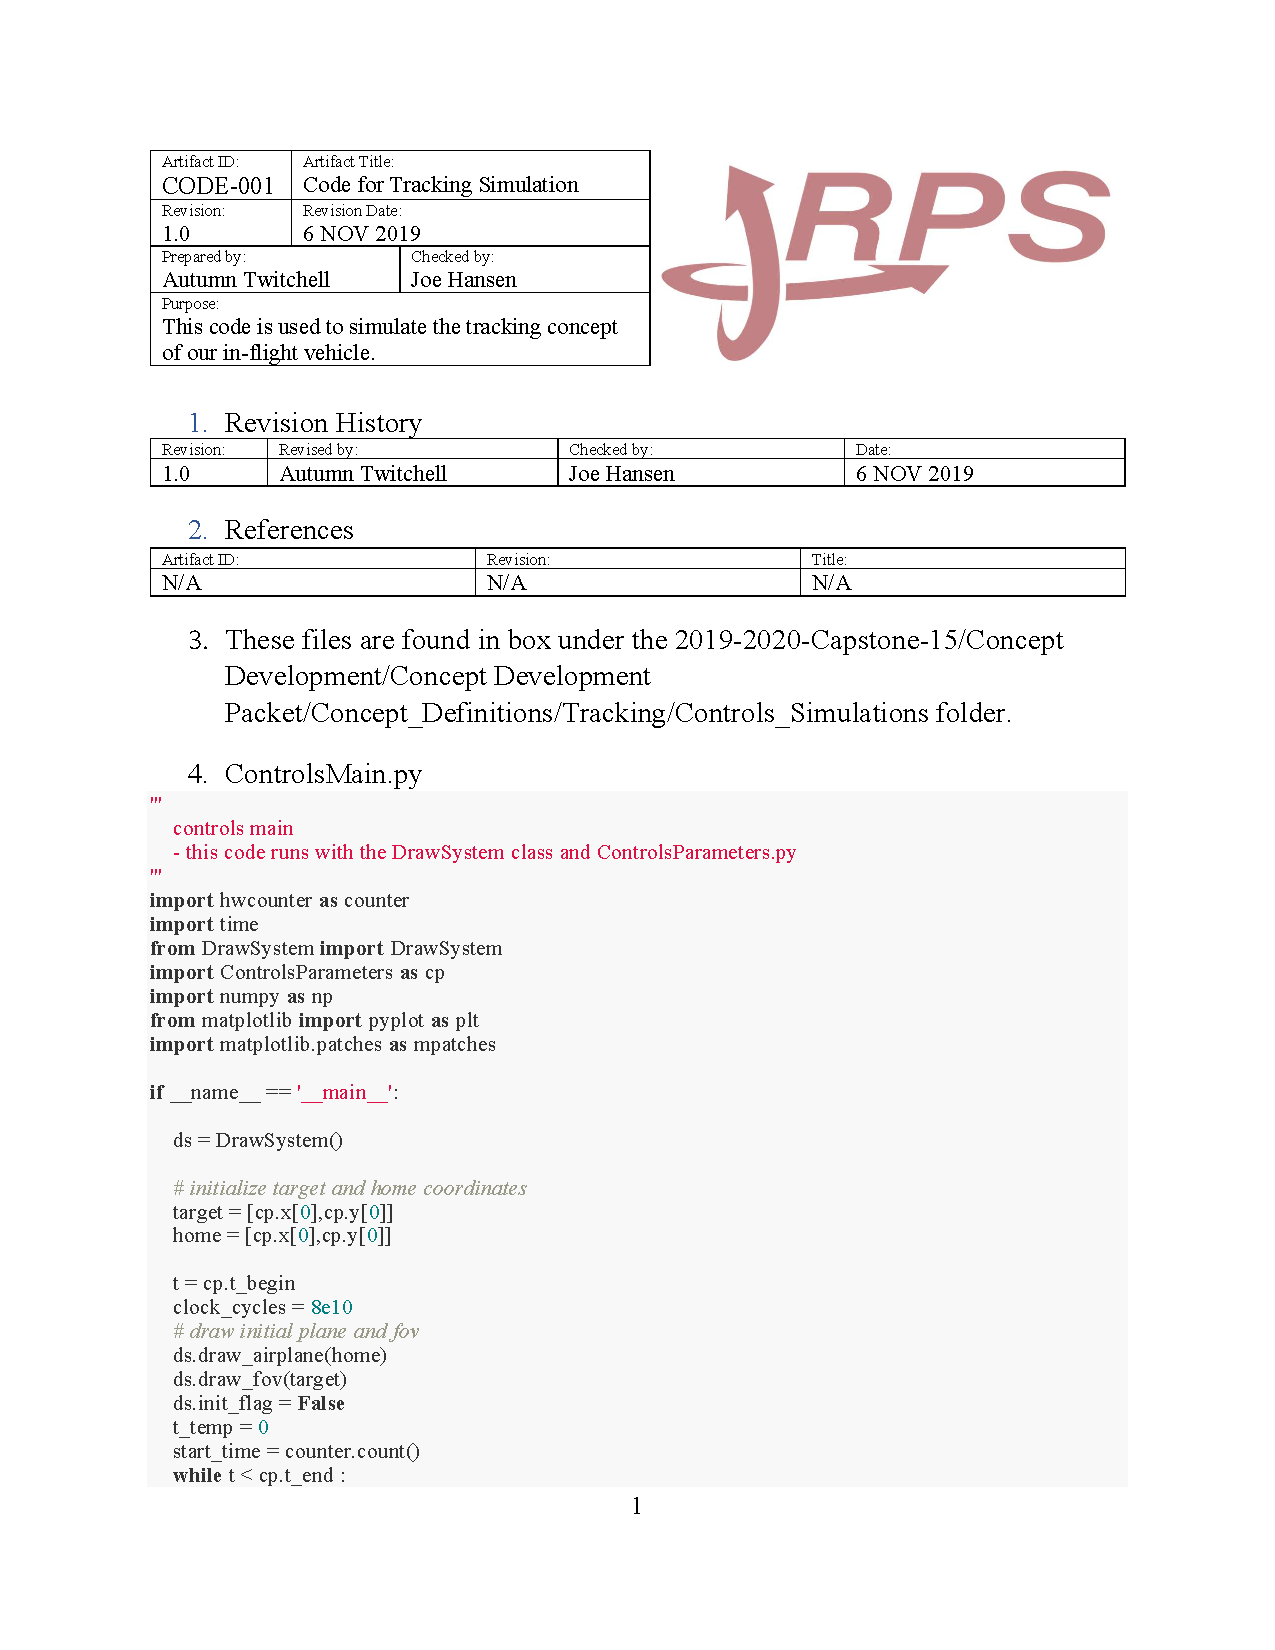
\includepdf[pages=-]{Artifacts/CODE-001-CodeForTrackingSimulation.pdf}  % Includes all pages of a pdf file

% \cleardoublepage  %%% Used if including pdf artifacts directly
\supportingartifact{TODO Team Objectives and Development Overview}  
%% To include a pdf file of the artifact, uncomment the line below, and put the name of the pdf in the correct spot.

\includepdf[pages=-]{Artifacts/TODO/TODO_for_CD.pdf}  % Includes all pages of a pdf file

\clearpage


\end{document}
